
\subsection{Introducción}
Durante el segundo sprint se continuó con el desarrollo de la integración 
de las aplicaciones mencionadas en el sprint anterior.
Para este sprint en especifico se trabajó en los detalles sobre los autores, 
asi como su red de coautoría, articulos publicados y topicos de interes.

\subsection{Objetivos}
\begin{itemize}
    \item Implementar las ventanas para cada uno de los detalles de los autores.
    \item Integrar la fuerza de colaboración entre autores.
    \item Desarrollar la funcionalidad de articulos publicados por autor.
    \item Enrutamiento para las diferentes vistas de los autores.
\end{itemize}

\subsection{Planificación}
Para este sprint se selecciono un total de 2 historias de usuario, divididas en un total de
12 tareas a realizar las cuales fueron asignadas a los integrantes del equipo de desarrollo.

En la Tabla \ref{C2T2:Historias de Usuario del Sprint 2} se detallan las historias de usuario seleccionadas para este sprint.

\begin{table}[H]
    \centering
    \begin{tabular}{|p{2.5cm}|p{5cm}|p{6cm}|}
        \midrule
        \textbf{Identificador} & \textbf{Historia de Usuario}                                                                                                                                                                               & \textbf{Tareas} \\
        \hline
        HU-SE-03 & Como usuario no registrado, deseo poder ver la red de coautoría de un autor para visualizar un grafo con los autores con los que ha colaborado, así como la fuerza de esas colaboraciones &
        \begin{compactitem}
            \item Diseñar e implementar la interfaz y el grafo interactivo
            \item Definir y aplicar un esquema visual para la fuerza de la colaboración
            \item Implementar funcionalidades interactivas y filtros
            \item Agregar un panel de detalles con información adicional sobre el autor
        \end{compactitem}
        \\
        \hline
        HU-SE-04 & Como usuario no registrado quiero poder ver los artículos de un investigador para conocer su trabajo y las publicaciones en las que ha contribuido &
        \begin{compactitem}
            \item Diseñar la interfaz y enrutamiento para la lista de artículos
            \item Implementar la tabla de artículos y la funcionalidad de redirección
        \end{compactitem}
        \\
        \hline
        
    \end{tabular}
    \caption{Historias de Usuario del sprint 2}
    \label{C2T2:Historias de Usuario del Sprint 2}
\end{table}


Al igual que en el sprint anterior, cada historia de usuario se dividió en tareas más pequeñas,
las cuales se asignaron a los integrantes del equipo de desarrollo. Asi también se definieron
los criterios de aceptación que se muestran en la Figura \ref{C2F2:Criterios de Aceptacion HU-SE-03} y en la Figura \ref{C2F2:Criterios de Aceptacion HU-SE-04}.
para cada una con el fin de asegurar la calidad del desarrollo y
que cada miembro del equipo tuviera claro lo que se esperaba de la tarea asignada.
%%Input the figure

\begin{figure}[H]
    \centering
    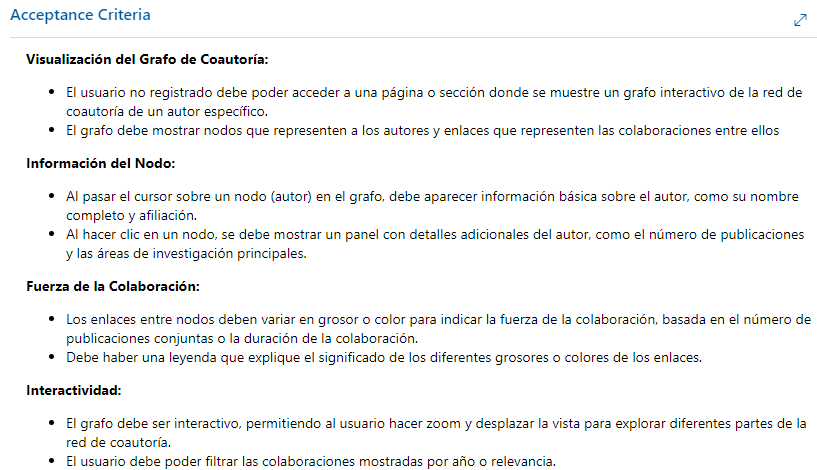
\includegraphics[width=0.8\textwidth]{../02Figures/02Chapter/Sprints/Sprint-2/aceptance-criteria-HU-SE-03.png}
    \caption{Criterios de Aceptación HU-SE-03}
    \label{C2F2:Criterios de Aceptacion HU-SE-03}
\end{figure}

\begin{figure}[H]
    \centering
    
\includegraphics[width=0.8\textwidth]{../02Figures/02Chapter/Sprints/Sprint-2/aceptance-criteria-HU-SE-04.png}
    \caption{Criterios de Aceptación HU-SE-04}
    \label{C2F2:Criterios de Aceptacion HU-SE-04}
\end{figure}

A continuación en la Figura \ref{fig:azure-board-sprint-2} se muestran las tareas de cada historia de usuario. Asi como en  Azure DevOps se crearon los \textit{work items} para cada tarea y se asignaron a los miembros del equipo.

\begin{figure}[H]
    \centering
    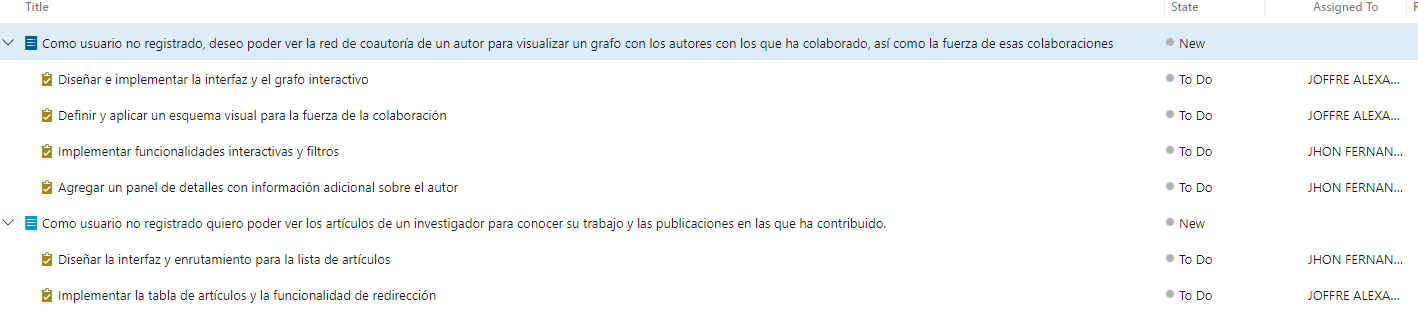
\includegraphics[width=1\textwidth]{../02Figures/02Chapter/Sprints/Sprint-2/fig_azure-board-sprint-2.png}
    \caption{Planificación de tareas del sprint 2}
    \label{fig:azure-board-sprint-2}
\end{figure}


\subsection{Implementación}
Al igual que el sprint anterior, se utilizó Figma para el diseño de los mockups de las vistas que posteriormente se implementarán utilizando Angular.
En la Figura \ref{fig:mobile-first-network} se muestra el diseño de la vista de los detalles de un autor. Así como los detalles que va tener su red de coautoría.

\begin{figure}[H]
    \centering
    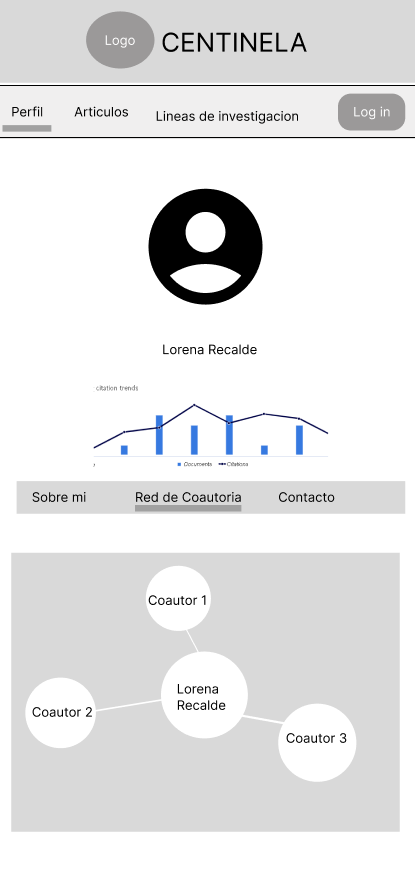
\includegraphics[scale=0.5]{../02Figures/02Chapter/Sprints/Sprint-2/mobile-first-network.png}
    \caption{Mockup de los detalles de un autor}
    \label{fig:mobile-first-network}
\end{figure}

Como se muestra en la Figura \ref{fig:mobile-first-network}, se diseñó la vista de los detalles de un autor, en la cual se muestra la red de coautoría del autor seleccionado. 
En la red de coautoría se muestra un grafo con los autores con los que ha colaborado, la fuerza de colaboración con cada autor se refleja en el grosor de la línea que los une.

En la Figura \ref{fig:mobile-first-articles} se muestra el diseño de la vista de los artículos publicados por un autor.
Los mismos estan representados en una tabla con la información de cada uno y contendran la interactividad que permitira al usuario redirigir al mockup de la Figura \ref{fig:mockup-article-detail}.

\begin{figure}[H]
    \centering
    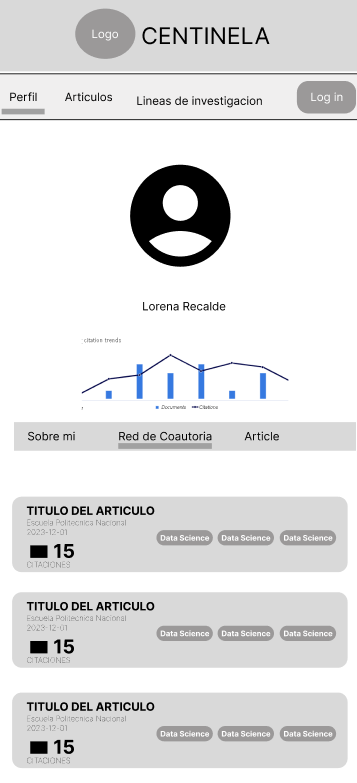
\includegraphics[scale=0.5]{../02Figures/02Chapter/Sprints/Sprint-2/mobile-first-articles.png}
    \caption{Mockup de los artículos publicados por un autor}
    \label{fig:mobile-first-articles}
\end{figure}

Para implementar la red de Coautoría se utilizó la librería D3.js, la cual permite la creación de gráficos interactivos en la web.
Para ello primero debemos definir los nodos y las relaciones entre ellos, en este caso los autores y la fuerza de colaboración entre ellos.
En la Figura \ref{fig:network-interface-ts} se muestra la interfaz en Typescript que servira para la creación de la red de coautoría.

\begin{figure}[H]
    \centering
    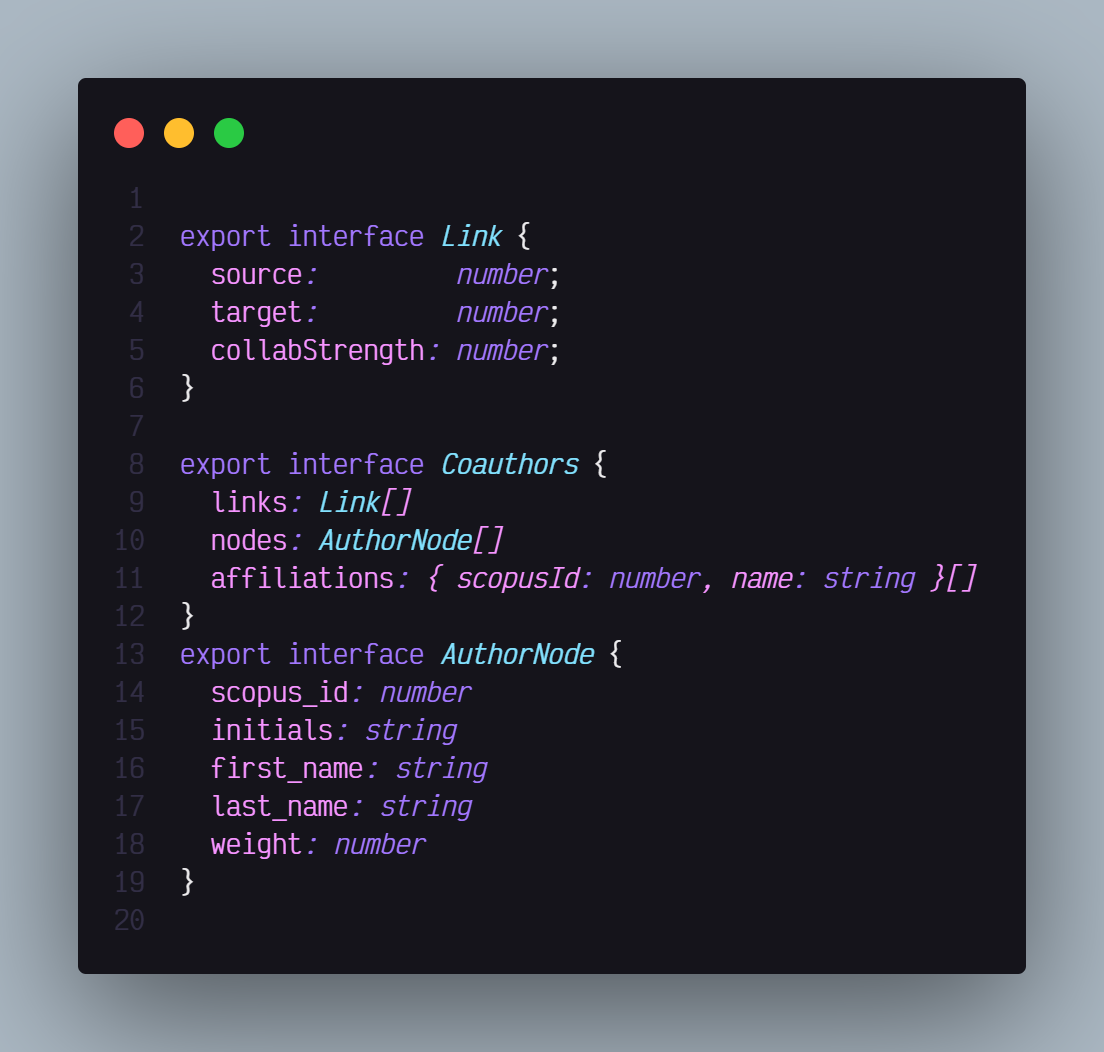
\includegraphics[scale=0.26]{../02Figures/02Chapter/Sprints/Sprint-2/coauthors-interface-typescript.png}
    \caption{Interfaz en Typescript para la creación de la red de coautoría}
    \label{fig:network-interface-ts}
\end{figure}

Debido a que el actual componente no se encargara de la creación de la red, sino que se encargará de la visualización de la misma. No se ahondará en la implementación de la red de coautoría, ya que se encuentra fuera del alcance de este documento.
El resultado final de la red de coautoría se muestra en la Figura \ref{fig:network-coauthors}.
\begin{figure}[H]
    \centering
    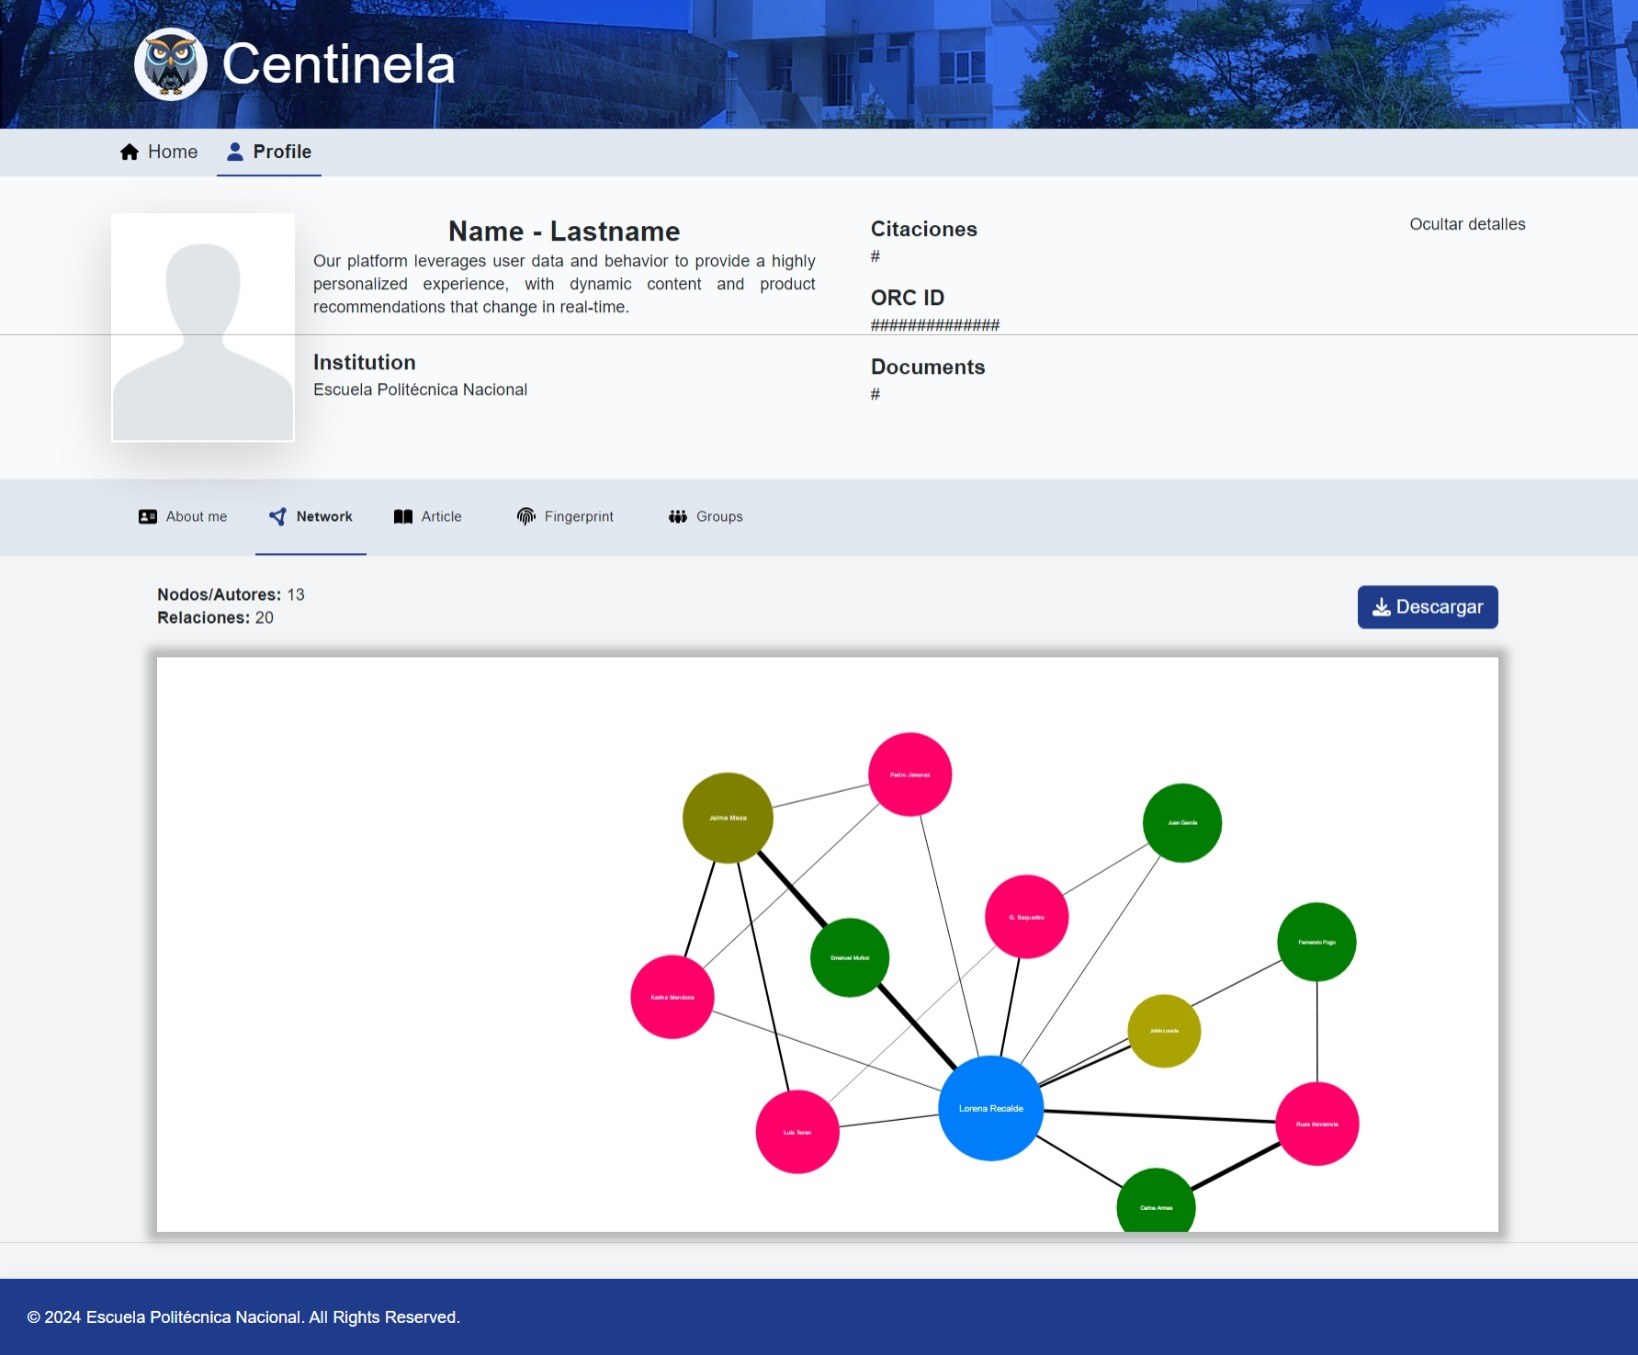
\includegraphics[scale=0.25]{../02Figures/02Chapter/Sprints/Sprint-2/network-coauthors.jpeg}
    \caption{Red de coautoría}
    \label{fig:network-coauthors}
\end{figure}

Cabe mencionar que para armar la red de coautoría que se muestra en la Figura \ref{fig:network-coauthors} se utilizó un conjunto de datos de prueba, ya que  de momento la aplicación no cuenta con la información necesaria para armar la red de coautoría.

Ahora en la Figura \ref{fig:articles-table} se muestra la tabla de los artículos publicados por un autor. Esta tabla también contendrá la interactividad que permitirá al usuario redirigir al mockup de la Figura \ref{fig:mockup-article-detail}.
\begin{figure}[H]
    \centering
    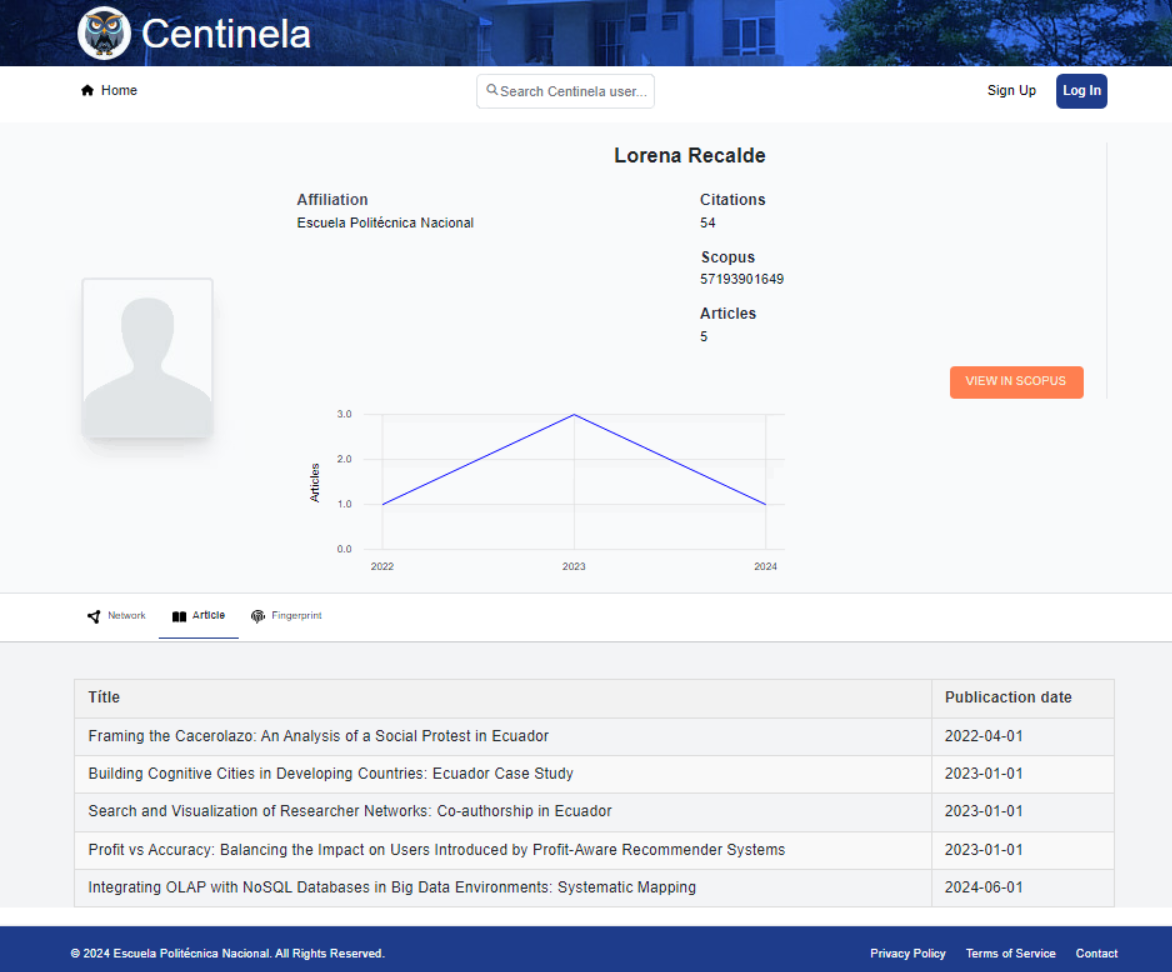
\includegraphics[scale=0.5]{../02Figures/02Chapter/Sprints/Sprint-2/article-table.png}
    \caption{Tabla de artículos publicados por un autor}
    \label{fig:articles-table}
\end{figure}

Para el despliegue de la aplicación en este sprint se utilizo Render como plataforma de despliegue, la cual permite el despliegue de aplicaciones web de forma gratuita.
En la Figura \ref{fig:render-deploy} se muestra el despliegue de la aplicación en Render.

%
%\begin{figure}[H]
%    \centering
%    \includegraphics[scale=0.5]{../02Figures/02Chapter/Sprints/Sprint-2/render-deploy.png}
%    \caption{Despliegue de la aplicación en Render}
%    \label{fig:render-deploy}
%\end{figure}

\subsection{Revisión y Retrospectiva}
Como resultado de este sprint se logró implementar las ventanas para cada uno de los detalles de los autores, la integración de la fuerza de colaboración entre autores, la funcionalidad de los artículos publicados por autor y el enrutamiento para las diferentes vistas de los autores.
Se logró cumplir con los objetivos planteados para este sprint, sin embargo, se presentaron algunos problemas durante el desarrollo de las tareas asignadas.
Uno de los problemas que se presentó fue la falta de información necesaria para la creación de la red de coautoría, ya que la aplicación no cuenta con la información necesaria para armar la red de coautoría.
Debido a que la implementación de la extracción de la información desde scopus se realizará en el siguiente sprint, sin embargo los servicios que se encargan de construir la red de coautoría ya se encuentran implementados y listos para recibir la información necesaria.

Al igual que en el Sprint anterior, las tareas relacionadas con la integración con Scopus quedaron pendientes, ya que se decidió que la implementación de la extracción de la información desde Scopus se realizará iniciara en el siguiente Sprint.